\ifdefined\inMainDoc\else
\documentclass[12pt,a4paper]{article}
% ================================================================
%  PRÉAMBULE COMMUN - ANNALES CORRIGÉES
%  Université de Kara - FaST - Licence Fondamentale MPC
%  Design optimisé impression noir et blanc
% ================================================================

% -- ENCODAGE & LANGUE --
\usepackage[utf8]{inputenc}
\usepackage[T1]{fontenc}
\usepackage[french]{babel}
\usepackage{lmodern}
\usepackage{microtype}

% -- MISE EN PAGE --
\usepackage[a4paper, top=2.8cm, bottom=2.5cm, left=2.5cm, right=2.5cm, headheight=14pt]{geometry}
\usepackage{setspace}
\setstretch{1.2}
\usepackage{parskip}
\setlength{\parindent}{1.2em}
\setlength{\parskip}{4pt}

% -- MATHS --
\usepackage{amsmath, amssymb, mathtools, amsthm}
\usepackage{mathrsfs}
\usepackage{dsfont}
\usepackage{bm}
\usepackage{cancel}
\usepackage{textcomp}
% Définition de \oiint (intégrale de surface fermée) sans package supplémentaire
\newcommand{\oiint}{\mathop{\iint\!\!\!\!\!\!\!\bigcirc}\limits}

% -- PHYSIQUE & CHIMIE --
\usepackage{physics}
\usepackage{siunitx}
% Lorsque physics est chargé, siunitx omet \qty. On le restaure ici :
\AtBeginDocument{\RenewCommandCopy\qty\SI}
\sisetup{locale = FR, detect-all, output-decimal-marker={,}}
% Commande de substitution pour les unités posant problème avec pdflatex
% (ohm, degreeCelsius, micro, angstrom, percent utilisent des caractères non-ASCII)
\newcommand{\qtyohm}[1]{\ensuremath{\num{#1}\,\Omega}}
\newcommand{\qtydegc}[1]{\ensuremath{\num{#1}\,{}^\circ\text{C}}}
\newcommand{\qtyangstrom}[1]{\ensuremath{\num{#1}\,\text{\AA}}}
\newcommand{\qtypercent}[1]{\ensuremath{\num{#1}\,\%}}
\newcommand{\qtyum}[1]{\ensuremath{\num{#1}\,\mu\text{m}}}
\usepackage[version=4]{mhchem}

% -- GRAPHISMES --
\usepackage{graphicx}
\usepackage{float}
\usepackage{caption}
\usepackage{subcaption}
\usepackage{wrapfig}
\usepackage{tikz}
\usetikzlibrary{calc, arrows.meta, patterns, shapes.geometric}
\usepackage{pgfplots}
\pgfplotsset{compat=1.18}

% -- TABLEAUX --
\usepackage{booktabs}
\usepackage{array}
\usepackage{tabularx}
\usepackage{multirow}

% -- LISTES --
\usepackage{enumitem}
\setlist[enumerate]{topsep=3pt, itemsep=2pt, parsep=0pt}
\setlist[itemize]{topsep=3pt, itemsep=2pt, parsep=0pt, label={.}}

% -- BOÎTES (noir et blanc) --
\usepackage{mdframed}
\usepackage{tcolorbox}
\tcbuselibrary{skins, breakable, theorems}

% Boîte EXERCICE : encadré avec filet épais, fond blanc
\newmdenv[
  linewidth=1.2pt,
  linecolor=black,
  roundcorner=3pt,
  skipabove=10pt,
  skipbelow=6pt,
  innertopmargin=8pt,
  innerbottommargin=8pt,
  innerleftmargin=10pt,
  innerrightmargin=10pt,
  backgroundcolor=white,
  frametitle={\bfseries\small Exercice},
  frametitlealignment=\raggedright,
  frametitleaboveskip=4pt,
  frametitlebelowskip=4pt,
]{boiteexercice}

% Boîte CORRIGÉ : fond gris très clair + filet fin
\newmdenv[
  linewidth=0.6pt,
  linecolor=black,
  leftline=true,
  rightline=false,
  topline=false,
  bottomline=false,
  linecolor=black,
  innerleftmargin=12pt,
  innerrightmargin=8pt,
  innertopmargin=6pt,
  innerbottommargin=6pt,
  backgroundcolor=gray!8,
  skipabove=4pt,
  skipbelow=8pt,
]{boitecorrige}

% Boîte RÉSUMÉ DE COURS : double encadré
\newmdenv[
  linewidth=0.8pt,
  linecolor=black,
  roundcorner=2pt,
  backgroundcolor=gray!12,
  innertopmargin=10pt,
  innerbottommargin=10pt,
  innerleftmargin=12pt,
  innerrightmargin=12pt,
  skipabove=12pt,
  skipbelow=8pt,
]{boiteresume}

% Boîte ATTENTION/REMARQUE : barre gauche épaisse
\newmdenv[
  leftline=true,
  rightline=false,
  topline=false,
  bottomline=false,
  linewidth=3pt,
  linecolor=black,
  backgroundcolor=gray!5,
  innerleftmargin=12pt,
  innerrightmargin=8pt,
  innertopmargin=5pt,
  innerbottommargin=5pt,
  skipabove=6pt,
  skipbelow=6pt,
]{boiteremarque}

% -- DIFFICULTÉ DES EXERCICES --
\newcommand{\facile}{$\star$}
\newcommand{\moyen}{$\star\!\star$}
\newcommand{\difficile}{$\star\!\star\!\star$}
\newcommand{\niveau}[1]{\hfill\textbf{#1}\hspace{2pt}}

% -- EN-TÊTES ET PIEDS DE PAGE --
\usepackage{fancyhdr}
\pagestyle{fancy}
\fancyhf{}
\renewcommand{\headrulewidth}{0.5pt}
\renewcommand{\footrulewidth}{0.3pt}

% -- HYPERLIENS --
\usepackage[hidelinks]{hyperref}
\hypersetup{
    colorlinks=false,
    pdftitle={Annale Corrigée - Licence MPC - Université de Kara}
}

% -- TITRES --
\usepackage{titlesec}
\titleformat{\section}{\Large\bfseries}{\thesection.}{0.8em}{}[\vspace{2pt}\hrule\vspace{4pt}]
\titleformat{\subsection}{\large\bfseries}{\thesubsection.}{0.7em}{}
\titleformat{\subsubsection}{\normalsize\bfseries}{\thesubsubsection.}{0.6em}{}

% -- THÉORÈMES --
\theoremstyle{definition}
\newtheorem{defn}{Définition}[section]
\newtheorem{prop}{Propriété}[section]
\newtheorem{thm}{Théorème}[section]
\newtheorem{corol}{Corollaire}[section]
\newtheorem{exemple}{Exemple}[section]

% -- COMMANDES MATHÉMATIQUES UTILES --
\newcommand{\vect}[1]{\overrightarrow{#1}}
\newcommand{\R}{\mathbb{R}}
\newcommand{\N}{\mathbb{N}}
\newcommand{\Z}{\mathbb{Z}}
\newcommand{\C}{\mathbb{C}}
\renewcommand{\d}{\mathrm{d}}
\newcommand{\deriv}[2]{\dfrac{\d #1}{\d #2}}
\newcommand{\dpart}[2]{\dfrac{\partial #1}{\partial #2}}
\newcommand{\rot}{\overrightarrow{\mathrm{rot}}\,}
\renewcommand{\div}{\mathrm{div}\,}
\renewcommand{\grad}{\overrightarrow{\mathrm{grad}}\,}
\newcommand{\e}{\mathrm{e}}
\newcommand{\ii}{\mathrm{i}}
\renewcommand{\Tr}{\mathrm{Tr}}

% Numérotation des équations par section
\numberwithin{equation}{section}

% -- RÉSULTATS ENCADRÉS --
\newcommand{\res}[1]{\[\boxed{#1}\]}

% -- REMARQUE INLINE --
\newcommand{\rmq}[1]{\begin{boiteremarque}\textbf{Remarque.} #1\end{boiteremarque}}

% -- MISE EN VALEUR DU RÉSULTAT FINAL --
\newcommand{\reponse}[1]{%
  \begin{center}
    \fbox{\begin{minipage}{0.92\textwidth}\centering #1\end{minipage}}
  \end{center}%
}


\lhead{\small\textit{Mécanique Quantique - Licence 2}}
\rhead{\small\textit{FaST, Université de Kara}}
\cfoot{\thepage}

\begin{document}
\fi

\begin{center}
  {\LARGE\bfseries INTRODUCTION À LA MÉCANIQUE QUANTIQUE}\\[0.3cm]
  {\normalsize Licence 2 - Mathématiques, Physique et Chimie}\\[0.1cm]
  \rule{0.7\textwidth}{0.8pt}
\end{center}

\section*{Résumé du cours}

\begin{boiteresume}

\textbf{1. Dualité onde-corpuscule - Relations de de Broglie.}
À toute particule de quantité de mouvement $p$ et d'énergie $E$ on associe une onde de longueur
d'onde $\lambda$ et de fréquence $\nu$ :
\[
  \lambda = \frac{h}{p}, \qquad E = h\nu = \hbar\omega.
\]
Constantes fondamentales : $h = \qty{6.626e-34}{J.s}$, $\hbar = h/(2\pi)$,
$k_B = \qty{1.381e-23}{J.K^{-1}}$, $c = \qty{3e8}{m.s^{-1}}$.

\textbf{2. Fonction d'onde et interprétation probabiliste.}
L'état d'un système est décrit par une fonction d'onde $\Psi(x,t)$. La densité de probabilité de
présence est $\rho(x,t) = |\Psi(x,t)|^2$. La condition de normalisation impose :
\[
  \int_{-\infty}^{+\infty} |\Psi(x,t)|^2 \, dx = 1.
\]

\textbf{3. Équation de Schrödinger.}

\textit{Dépendante du temps} :
\[
  i\hbar\frac{\partial\Psi}{\partial t} = \hat{H}\Psi =
  \left[-\frac{\hbar^2}{2m}\frac{\partial^2}{\partial x^2} + V(x)\right]\Psi.
\]

\textit{Stationnaire} (états d'énergie définie, $\Psi = \psi(x)\,e^{-iEt/\hbar}$) :
\[
  \hat{H}\psi = E\psi, \qquad
  -\frac{\hbar^2}{2m}\frac{d^2\psi}{dx^2} + V(x)\psi = E\psi.
\]

\textbf{4. Puits infini de potentiel (particule en boîte).}
Pour une particule confinée dans $[0,L]$ avec $V=0$ à l'intérieur et $V=+\infty$ à l'extérieur :
\[
  E_n = \frac{n^2\pi^2\hbar^2}{2mL^2}, \qquad
  \psi_n(x) = \sqrt{\frac{2}{L}}\sin\!\left(\frac{n\pi x}{L}\right), \qquad n = 1, 2, 3, \ldots
\]
Les niveaux d'énergie sont quantifiés ; $E_1$ est l'énergie de point zéro.

\textbf{5. Opérateurs et observables.}
À toute observable est associé un opérateur hermitien $\hat{A}$. Les valeurs propres de $\hat{A}$
sont les seuls résultats de mesure possibles. La valeur moyenne est :
\[
  \langle\hat{A}\rangle = \int\Psi^*\hat{A}\Psi\,dx.
\]
Opérateur position : $\hat{x} = x$. Opérateur impulsion : $\hat{p} = -i\hbar\,\partial/\partial x$.

\textbf{6. Principe d'incertitude de Heisenberg.}
Pour toute paire position-impulsion :
\[
  \Delta x \cdot \Delta p \geq \frac{\hbar}{2}.
\]
L'égalité est atteinte pour les paquets d'ondes gaussiens (états cohérents).

\textbf{7. Modèle de Bohr de l'atome d'hydrogène (hydrogénoïdes).}
Quantification du moment cinétique : $|L| = n\hbar$, $n\geq 1$. Rayons et énergies des orbites :
\[
  r_n = \frac{n^2}{Z}a_0, \quad a_0 = \frac{4\pi\varepsilon_0\hbar^2}{me^2} \approx \qtyangstrom{0.529}.
  \qquad E_n = -\frac{Z^2}{n^2}E_1, \quad E_1 = \qty{13.6}{eV}.
\]
Série spectrale : $\dfrac{1}{\lambda_{np}} = Z^2 R_H\!\left(\dfrac{1}{p^2}-\dfrac{1}{n^2}\right)$,
$R_H \approx \qty{1.097e7}{m^{-1}}$.

\end{boiteresume}

\newpage
\section{Rayonnement du corps noir - Loi de Planck}

\subsection*{Exercice 1 - Loi de Planck et loi de Wien \niveau{\moyen}}

\begin{boiteexercice}
\begin{enumerate}
  \item Écrire l'expression de la loi de Planck donnant la densité spectrale d'énergie en fonction
    de la fréquence $\nu$. Interpréter cette loi.
  \item Exprimer la loi de Planck en fonction de la longueur d'onde $\lambda$. En déduire la loi de
    déplacement de Wien et la valeur de la constante $C_0$ (on posera $x = hc/(\lambda k_BT)$).
    On donne : la solution de $x/5 = 1-e^{-x}$ est $x_0 = 4{,}965$.
  \item Applications :
    \begin{enumerate}
      \item Le spectre solaire présente un maximum pour $\lambda_M = \qtyum{0.55}$. Estimer
        la température à la surface du Soleil, assimilé à un corps noir.
      \item À quelle longueur d'onde se situe le maximum de rayonnement du corps humain
        (température $T_H \approx \qtydegc{37}$, assimilé à un corps noir) ?
    \end{enumerate}
\end{enumerate}
\end{boiteexercice}

\begin{boitecorrige}
\textbf{1. Loi de Planck en fréquence.}
La densité spectrale volumique d'énergie d'un corps noir à la température $T$ vaut :
\[
  u(\nu, T) = \frac{8\pi h\nu^3}{c^3}\cdot\frac{1}{e^{h\nu/(k_BT)}-1}.
\]
Cette expression traduit deux effets. D'une part, la densité d'états électromagnétiques en
fréquence vaut $8\pi\nu^2/c^3$ (facteur purement ondulatoire). D'autre part, chaque mode
d'oscillation contient en moyenne une énergie $h\nu/(e^{h\nu/k_BT}-1)$, qui est le résultat de la
quantification de Planck : l'énergie est échangée par quanta discrets $h\nu$. Aux basses fréquences
on retrouve la loi de Rayleigh-Jeans ($u\propto\nu^2 T$) et aux hautes fréquences la loi de Wien
($u\propto e^{-h\nu/k_BT}$).

\textbf{2. Loi de Planck en longueur d'onde et loi de Wien.}
En utilisant $\nu = c/\lambda$ et $|d\nu| = (c/\lambda^2)|d\lambda|$, on passe à la densité
spectrale en longueur d'onde $u(\lambda,T) = u(\nu,T)\cdot c/\lambda^2$ :
\[
  u(\lambda, T) = \frac{8\pi hc}{\lambda^5}\cdot\frac{1}{e^{hc/(\lambda k_BT)}-1}.
\]

On cherche le maximum en $\lambda$ en annulant $\partial u/\partial\lambda = 0$.
En calculant $\partial\ln u/\partial\lambda = 0$ :
\[
  -\frac{5}{\lambda} + \frac{hc}{\lambda^2 k_BT}\cdot\frac{e^{x}}{e^{x}-1} = 0,
  \quad \text{avec } x = \frac{hc}{\lambda k_BT}.
\]
En multipliant par $\lambda/x$, on obtient $x/5 = 1 - e^{-x}$.
La solution est $x_0 = 4{,}965$, d'où la loi de déplacement de Wien :
\[
  \lambda_M T = \frac{hc}{x_0 k_B} = \frac{hc}{4{,}965\,k_B}.
\]
Numériquement :
\[
  C_0 = \frac{6{,}626\times10^{-34}\times3\times10^{8}}{4{,}965\times1{,}381\times10^{-23}}
      \approx \boxed{\qty{2.898e-3}{m.K}.}
\]

\textbf{3. a) Température à la surface du Soleil.}
\[
  T_\odot = \frac{C_0}{\lambda_M} = \frac{2{,}898\times10^{-3}}{0{,}55\times10^{-6}}
           \approx \qty{5269}{K} \approx \qtydegc{5000}.
\]
La surface du Soleil est à environ $\qty{5270}{K}$.

\textbf{3. b) Corps humain.}
La température du corps humain est $T_H = 37+273 = \qty{310}{K}$.
\[
  \lambda_M = \frac{C_0}{T_H} = \frac{2{,}898\times10^{-3}}{310}
            \approx \boxed{\qtyum{9.35}.}
\]
Cette longueur d'onde se situe dans l'infrarouge moyen, ce qui explique la détection par caméras
thermiques.
\end{boitecorrige}

\subsection*{Exercice 2 - Critère classique ou quantique \niveau{\facile}}

\begin{boiteexercice}
Dans chacun des cas suivants, préciser si l'on doit recourir à la mécanique quantique, en
comparant le quantum d'action $\mathcal{A}$ à la constante de Planck $h$.
\begin{enumerate}
  \item Une montre à ressort avec des pièces mobiles de taille $d \approx \qty{0.1}{mm}$,
    de masse $m \approx \qty{0.1}{mg}$ et de temps caractéristique $t \approx \qty{1}{s}$.
  \item Un noyau atomique d'énergie de liaison par nucléon $E \approx \qty{8}{MeV}$,
    de rayon $r \approx \qty{1}{fm}$ et de masse $m \approx \qty{1.6e-27}{kg}$.
\end{enumerate}
\end{boiteexercice}

\begin{boitecorrige}
Le critère est le suivant : si $\mathcal{A} \gg h$, la mécanique classique suffit ; si
$\mathcal{A} \lesssim h$, la mécanique quantique est nécessaire.

\textbf{1. Montre à ressort.}
On estime le quantum d'action par $\mathcal{A} = md^2/t$ :
\[
  \mathcal{A} = \frac{(10^{-4})^2 \times 10^{-7}}{1} = 10^{-15}\;\text{J·s}.
\]
Puisque $h \approx 6{,}6\times10^{-34}\;\text{J·s}$, on a $\mathcal{A} \approx 10^{18}h \gg h$.
La mécanique classique est largement suffisante.

\textbf{2. Noyau atomique.}
On estime $\mathcal{A} = r\sqrt{mE}$ :
\[
  E = 8\times10^6 \times 1{,}6\times10^{-19} = 1{,}28\times10^{-12}\;\text{J}.
\]
\[
  \mathcal{A} = 10^{-15}\times\sqrt{1{,}6\times10^{-27}\times1{,}28\times10^{-12}}
              \approx 10^{-15}\times 1{,}43\times10^{-19} \approx 1{,}4\times10^{-34}\;\text{J·s}.
\]
On a $\mathcal{A} \approx 0{,}2\,h \lesssim h$. La mécanique quantique est indispensable pour
décrire la physique nucléaire.
\end{boitecorrige}

\newpage
\section{Atome d'hydrogène et modèle de Bohr}

\subsection*{Exercice 3 - Atome hydrogénoïde \niveau{\moyen}}

\begin{boiteexercice}
Un hydrogénoïde est un atome constitué d'un électron (masse $m$, charge $-e$) et d'un noyau de
charge $+Ze$, supposé fixe. L'électron décrit un cercle de rayon $r$ autour du noyau.
\begin{enumerate}
  \item \textbf{a)} Montrer que l'énergie totale de l'électron s'écrit $E = -\dfrac{Ze^2}{8\pi\varepsilon_0 r}$.\\
        \textbf{b)} Que signifie physiquement une énergie totale nulle ?
  \item Que donne la mécanique classique pour le mouvement de l'électron ?
  \item En appliquant les deux hypothèses de Bohr :
    \begin{itemize}
      \item Les orbites permises vérifient $|L| = n\hbar$, $n \geq 1$.
      \item L'électron émet un photon de fréquence $\nu_{np} = (E_n-E_p)/h$ lors d'une transition
        $n \to p$ ($n > p$).
    \end{itemize}
    \textbf{a)} Établir l'expression du rayon $r_n$ et de
    l'énergie $E_n$ des orbites permises.

    \textbf{b)} Montrer que les longueurs d'onde d'émission vérifient :
    \[
    \dfrac{1}{\lambda_{np}} = Z^2 R_H\!\left(\dfrac{1}{p^2}-\dfrac{1}{n^2}\right).
    \]
    Exprimer et calculer $R_H$.
\end{enumerate}
\end{boiteexercice}

\begin{boitecorrige}
\textbf{1. a)} L'énergie potentielle d'interaction coulombienne est :
\[
  E_p = -\frac{Ze^2}{4\pi\varepsilon_0 r}.
\]
La condition d'équilibre sur l'orbite circulaire (force centripète = force coulombienne) donne :
\[
  \frac{mv^2}{r} = \frac{Ze^2}{4\pi\varepsilon_0 r^2}
  \implies E_c = \frac{1}{2}mv^2 = \frac{Ze^2}{8\pi\varepsilon_0 r}.
\]
L'énergie totale vaut donc :
\[
  \boxed{E = E_c + E_p = \frac{Ze^2}{8\pi\varepsilon_0 r} - \frac{Ze^2}{4\pi\varepsilon_0 r}
          = -\frac{Ze^2}{8\pi\varepsilon_0 r} < 0.}
\]

\textbf{1. b)} $E = 0$ correspond à $r\to\infty$ : l'électron est infiniment éloigné du noyau et
n'est plus lié à lui. Cela représente l'ionisation de l'atome.

\textbf{2.} En mécanique classique, la force coulombienne étant attractive et l'électron en
mouvement, il rayonne de l'énergie électromagnétique (accélération centripète). Il perd ainsi de
l'énergie, son rayon d'orbite diminue continûment et il finit par s'effondrer sur le noyau en un
temps très court (estimé à $\approx \qty{e-11}{s}$). La mécanique classique prédit donc un atome
instable, ce qui contredit l'observation.

\textbf{3. a) Orbites permises.}
La quantification du moment cinétique $mvr = n\hbar$, combinée à la condition d'équilibre
$mv^2 = Ze^2/(4\pi\varepsilon_0 r)$, donne :
\[
  v = \frac{n\hbar}{mr} \implies m\frac{n^2\hbar^2}{m^2r^2} = \frac{Ze^2}{4\pi\varepsilon_0 r}
  \implies r_n = \frac{4\pi\varepsilon_0\hbar^2}{me^2}\cdot\frac{n^2}{Z} = \frac{n^2}{Z}a_0,
\]
avec $a_0 = 4\pi\varepsilon_0\hbar^2/(me^2) \approx \qtyangstrom{0.529}$ (rayon de Bohr).
L'énergie correspondante :
\[
  \boxed{E_n = -\frac{Ze^2}{8\pi\varepsilon_0 r_n} = -\frac{Z^2 me^4}{32\pi^2\varepsilon_0^2\hbar^2}
              \cdot\frac{1}{n^2} = -\frac{Z^2}{n^2}E_1, \quad E_1 = \qty{13.6}{eV}.}
\]

\textbf{3. b) Séries spectrales.}
L'énergie du photon émis lors de la transition $n\to p$ :
\[
  h\nu_{np} = E_n - E_p = Z^2E_1\!\left(\frac{1}{p^2}-\frac{1}{n^2}\right).
\]
Puisque $\lambda = c/\nu$ :
\[
  \frac{1}{\lambda_{np}} = \frac{\nu_{np}}{c} = \frac{Z^2E_1}{hc}\!\left(\frac{1}{p^2}-\frac{1}{n^2}\right)
  = Z^2R_H\!\left(\frac{1}{p^2}-\frac{1}{n^2}\right),
\]
avec la constante de Rydberg :
\[
  R_H = \frac{E_1}{hc} = \frac{me^4}{8\varepsilon_0^2 h^3 c}
      \approx \boxed{\qty{1.097e7}{m^{-1}}.}
\]
\end{boitecorrige}

\newpage
\section{Fonction d'onde et principe d'incertitude}

\subsection*{Exercice 4 - Paquet d'ondes gaussien \niveau{\difficile}}

\begin{boiteexercice}
On considère une particule libre de masse $m$ décrite par un paquet d'ondes à une dimension, obtenu
par superposition d'ondes planes $e^{ikx}$ d'amplitude $g(k)$, où :
\[
  g(k) = \left(\frac{a^2}{2\pi}\right)^{1/4}\exp\!\left[-\frac{a^2}{4}(k-k_0)^2\right].
\]
$a$ est une constante de dimension d'une longueur et $k_0$ le vecteur d'onde central.
\begin{enumerate}
  \item \textbf{a)} Déterminer $\Psi(x,0)$.\\
        \textbf{b)} Calculer la densité de probabilité $|\Psi(x,0)|^2$ et la représenter schématiquement.
  \item Sachant que la largeur d'une gaussienne $f(\ell) = e^{-\ell^2/b^2}$ est $\Delta\ell = b/\sqrt{2}$ :
    \begin{enumerate}
      \item Calculer $\Delta x$ et $\Delta k$ correspondant à $|\Psi(x,0)|^2$ et $|g(k)|^2$.
      \item Évaluer le produit $\Delta x\cdot\Delta p$ et conclure.
    \end{enumerate}
\end{enumerate}
On donne : $\displaystyle\int_{-\infty}^{+\infty} e^{-\gamma y^2}\,dy = \sqrt{\pi/\gamma}$.
\end{boiteexercice}

\begin{boitecorrige}
\textbf{1. a) Calcul de $\Psi(x,0)$.}
\[
  \Psi(x,0) = \frac{1}{\sqrt{2\pi}}\int_{-\infty}^{+\infty}g(k)\,e^{ikx}\,dk.
\]
On substitue $g(k)$ et on complète le carré dans l'exposant, en posant $u = k-k_0$ :
\begin{align*}
  \Psi(x,0) &= \frac{1}{\sqrt{2\pi}}\left(\frac{a^2}{2\pi}\right)^{1/4}
               \int_{-\infty}^{+\infty}
               e^{-\frac{a^2}{4}u^2 + i(u+k_0)x}\,du\\
             &= \frac{e^{ik_0x}}{\sqrt{2\pi}}\left(\frac{a^2}{2\pi}\right)^{1/4}
               \int_{-\infty}^{+\infty}
               e^{-\frac{a^2}{4}\!\left(u - \frac{2ix}{a^2}\right)^2 - \frac{x^2}{a^2}}\,du.
\end{align*}
L'intégrale gaussienne (déplacée dans le plan complexe, résultat valable par prolongement
analytique) vaut $\sqrt{\pi/(a^2/4)} = 2\sqrt{\pi}/a$. Donc :
\[
  \Psi(x,0) = \frac{e^{ik_0x}}{\sqrt{2\pi}}\left(\frac{a^2}{2\pi}\right)^{1/4}
               e^{-x^2/a^2}\cdot\frac{2\sqrt{\pi}}{a}
            = \frac{1}{\sqrt{a}}\left(\frac{2}{\pi}\right)^{1/4}e^{ik_0x - x^2/a^2}.
\]
\[
  \boxed{\Psi(x,0) = \frac{1}{\sqrt{a}}\left(\frac{2}{\pi}\right)^{1/4}
         \exp\!\left(ik_0x - \frac{x^2}{a^2}\right).}
\]

\textbf{1. b) Densité de probabilité.}
\[
  |\Psi(x,0)|^2 = \frac{1}{a}\left(\frac{2}{\pi}\right)^{1/2}\exp\!\left(-\frac{2x^2}{a^2}\right).
\]
C'est une gaussienne centrée en $x=0$, de largeur caractéristique $a/\sqrt{2}$. Elle est
normalisée : $\int|\Psi|^2\,dx = 1$ (on le vérifie avec la formule donnée, $\gamma = 2/a^2$).

\begin{center}
\begin{tikzpicture}
  \begin{axis}[
    width=9cm, height=5cm,
    xlabel={$x$}, ylabel={$|\Psi(x,0)|^2$},
    xmin=-3.5, xmax=3.5,
    ymin=0,
    xtick={-2,0,2},
    xticklabels={$-a$, $0$, $a$},
    ytick=\empty,
    axis lines=left,
    samples=120,
    domain=-3.5:3.5,
  ]
    \addplot[black, thick] {exp(-2*x^2)};
  \end{axis}
\end{tikzpicture}
\end{center}

\textbf{2. a) Largeurs $\Delta x$ et $\Delta k$.}

Pour $|\Psi(x,0)|^2 = \dfrac{1}{a}\sqrt{\dfrac{2}{\pi}}\exp\!\left(-\dfrac{x^2}{(a/\sqrt{2})^2/2}\right)$
on identifie $b = a/\sqrt{2}$ (gaussienne en $e^{-2x^2/a^2} = e^{-x^2/b^2}$ avec $b = a/\sqrt{2}$),
d'où :
\[
  \Delta x = \frac{b}{\sqrt{2}} = \frac{a}{2}.
\]

Pour $|g(k)|^2 = \left(\dfrac{a^2}{2\pi}\right)^{1/2}\exp\!\left[-\dfrac{a^2}{2}(k-k_0)^2\right]$,
on identifie $b_k = \sqrt{2}/a$, d'où :
\[
  \Delta k = \frac{b_k}{\sqrt{2}} = \frac{1}{a}.
\]

\textbf{2. b) Produit des incertitudes.}
Puisque $p = \hbar k$, on a $\Delta p = \hbar\,\Delta k = \hbar/a$. Donc :
\[
  \Delta x\cdot\Delta p = \frac{a}{2}\cdot\frac{\hbar}{a} = \frac{\hbar}{2}.
\]
Le paquet d'ondes gaussien atteint la borne minimale du principe d'incertitude de Heisenberg
($\Delta x\cdot\Delta p = \hbar/2$). C'est un état cohérent, le plus localisé possible compatible
avec la mécanique quantique.
\end{boitecorrige}

\subsection*{Exercice 5 - Espace de Hilbert et bases orthonormées \niveau{\difficile}}

\begin{boiteexercice}
Soient $|e_1\rangle$, $|e_2\rangle$, $|e_3\rangle$ une base orthonormée d'un espace de Hilbert
$\mathcal{H}$ de dimension 3 sur $\mathbb{C}$. On considère :
\[
  |\Psi\rangle = \alpha(i|e_1\rangle + |e_2\rangle - |e_3\rangle),
  \qquad
  |\Phi\rangle = \beta(|e_2\rangle + |e_3\rangle).
\]
\begin{enumerate}
  \item Montrer que $\langle\Psi|\Phi\rangle = 0$ quels que soient $\alpha$ et $\beta$.
  \item Déterminer $\alpha$ et $\beta$ (à une phase près) tels que $\langle\Psi|\Psi\rangle =
    \langle\Phi|\Phi\rangle = 1$.
  \item Trouver un vecteur $|\chi\rangle$ tel que $\{|\chi\rangle, |\Psi\rangle, |\Phi\rangle\}$
    soit une base orthonormée de $\mathcal{H}$.
\end{enumerate}
\end{boiteexercice}

\begin{boitecorrige}
\textbf{1.}
\begin{align*}
  \langle\Psi|\Phi\rangle
  &= \alpha^*\beta\langle ie_1+e_2-e_3\,|\,e_2+e_3\rangle\\
  &= \alpha^*\beta\bigl(-i\langle e_1|e_2\rangle - i\langle e_1|e_3\rangle
     + \langle e_2|e_2\rangle + \langle e_2|e_3\rangle
     - \langle e_3|e_2\rangle - \langle e_3|e_3\rangle\bigr)\\
  &= \alpha^*\beta(0 + 0 + 1 + 0 - 0 - 1) = 0.
\end{align*}
Le résultat est nul quels que soient $\alpha$ et $\beta$ : les deux vecteurs sont orthogonaux.

\textbf{2.}
$\langle\Psi|\Psi\rangle = |\alpha|^2(|-i|^2 + 1^2 + 1^2) = 3|\alpha|^2 = 1
\implies |\alpha| = 1/\sqrt{3}$, soit $\alpha = e^{i\varphi}/\sqrt{3}$.

$\langle\Phi|\Phi\rangle = |\beta|^2(1+1) = 2|\beta|^2 = 1
\implies |\beta| = 1/\sqrt{2}$, soit $\beta = e^{i\psi}/\sqrt{2}$.

\textbf{3.}
On cherche $|\chi\rangle = a|e_1\rangle + b|e_2\rangle + c|e_3\rangle$ satisfaisant :
\begin{align*}
  \langle\Psi|\chi\rangle = 0 &\implies \alpha^*(-ia + b - c) = 0 \implies -ia+b-c=0,\\
  \langle\Phi|\chi\rangle = 0 &\implies \beta^*(b+c) = 0 \implies b+c=0,\\
  \langle\chi|\chi\rangle = 1 &\implies |a|^2+|b|^2+|c|^2 = 1.
\end{align*}
De $b+c=0$ on tire $c=-b$, puis $-ia+2b=0$, soit $a=2ib/(-1) = -2ib$... On reprend :
$-ia+b-(-b)=0 \implies -ia+2b=0 \implies a = 2b/i = -2ib$.

En posant $b = e^{i\theta}/\sqrt{6}$ (pour normaliser) :
$|a|^2+|b|^2+|c|^2 = 4|b|^2+|b|^2+|b|^2 = 6|b|^2 = 1 \implies |b|^2 = 1/6$.
\[
  \boxed{|\chi\rangle = \frac{e^{i\theta}}{\sqrt{6}}\bigl(-2i|e_1\rangle + |e_2\rangle - |e_3\rangle\bigr),
         \quad \theta\in\mathbb{R}.}
\]
\end{boitecorrige}

\newpage
\section{Puits de potentiel sphérique}

\subsection*{Exercice 6 - États liés à symétrie sphérique \niveau{\difficile}}

\begin{boiteexercice}
Une particule de masse $m$ est soumise au potentiel :
\[
  V(r) = \begin{cases} -V_0 & \text{si } r < a \\ 0 & \text{si } r > a \end{cases},
  \quad V_0 > 0.
\]
On s'intéresse aux états liés ($-V_0 < E < 0$) à symétrie sphérique ($\Psi = \Psi(r)$).
On rappelle : $\Delta\Psi(r) = \dfrac{1}{r}\dfrac{d^2}{dr^2}(r\Psi)$.

\begin{enumerate}
  \item Écrire l'équation de Schrödinger stationnaire dans les deux régions.
  \item Montrer que les solutions mathématiques sont $r\Psi_I = A\sin(\lambda r)+B\cos(\lambda r)$
    et $r\Psi_{II} = Ce^{-kr}+De^{kr}$. Exprimer $\lambda$ et $k$ en fonction de $E$, $V_0$, $m$,
    $\hbar$.
  \item \textbf{a)} Justifier que la solution physique en région II est $\Psi_{II} = Ce^{-kr}/r$.\\
        \textbf{b)} Justifier que la solution physique en région I est $\Psi_I = A\sin(\lambda r)/r$.
  \item \textbf{a)} Écrire les conditions de continuité en $r=a$.\\
        \textbf{b)} Montrer que les énergies $E$ satisfont $\cot(\lambda a) = -k/\lambda$.
\end{enumerate}
\end{boiteexercice}

\begin{boitecorrige}
\textbf{1. Équation de Schrödinger dans chaque région.}

En substituant $\Delta\Psi = \tfrac{1}{r}\tfrac{d^2}{dr^2}(r\Psi)$ :

\textit{Région I ($r < a$)} : $V = -V_0$, on pose $u = r\Psi$ :
\[
  -\frac{\hbar^2}{2m}\frac{d^2 u}{dr^2} - V_0 u = Eu
  \implies \frac{d^2 u}{dr^2} + \frac{2m(E+V_0)}{\hbar^2}u = 0.
\]

\textit{Région II ($r > a$)} : $V = 0$, on pose $u = r\Psi$ :
\[
  -\frac{\hbar^2}{2m}\frac{d^2 u}{dr^2} = Eu
  \implies \frac{d^2 u}{dr^2} - \frac{2m|E|}{\hbar^2}u = 0.
\]

\textbf{2. Forme des solutions.}
On pose $\lambda^2 = 2m(E+V_0)/\hbar^2 > 0$ (car $E > -V_0$) et $k^2 = 2m|E|/\hbar^2 > 0$
(car $E < 0$). Les équations différentielles donnent :
\[
  r\Psi_I = A\sin(\lambda r) + B\cos(\lambda r), \qquad
  r\Psi_{II} = Ce^{-kr} + De^{kr}.
\]

\textbf{3. a)} En région II, la condition de normalisation $\int_0^\infty|\Psi_{II}|^2 r^2\,dr < \infty$
impose que $e^{kr}/r$ soit intégrable, ce qui exige $D=0$. Donc $\Psi_{II}(r) = Ce^{-kr}/r$.

\textbf{3. b)} En région I, la fonction $\Psi_I = (A\sin\lambda r + B\cos\lambda r)/r$ doit être
finie en $r=0$. Or $\cos(\lambda r)/r \to \infty$ quand $r\to 0$. Donc on doit avoir $B=0$, et
$\Psi_I(r) = A\sin(\lambda r)/r$ (qui reste bien finie car $\sin(\lambda r)/r \to \lambda$ en
$r=0$).

\textbf{4. a) Conditions de continuité en $r=a$.}
La fonction d'onde et sa dérivée doivent être continues :
\[
  \Psi_I(a) = \Psi_{II}(a) : \quad \frac{A\sin(\lambda a)}{a} = \frac{Ce^{-ka}}{a}.
\]
\[
  \Psi_I'(a) = \Psi_{II}'(a) : \quad
  \frac{A\lambda\cos(\lambda a) - A\sin(\lambda a)/a}{1} = \frac{-Ce^{-ka}(k+1/a)}{1}.
\]
En pratique, on assure la continuité de $u = r\Psi$ et de $u'$ :
\[
  A\sin(\lambda a) = Ce^{-ka}, \qquad
  A\lambda\cos(\lambda a) = -kCe^{-ka}.
\]

\textbf{4. b) Équation de quantification.}
En divisant la seconde relation par la première :
\[
  \lambda\cot(\lambda a) = -k \implies \boxed{\cot(\lambda a) = -\frac{k}{\lambda}.}
\]
Cette équation transcendante détermine les valeurs permises de $\lambda$ (et donc de $E$). Elle
peut être résolue graphiquement en traçant $\cot(\lambda a)$ et $-k/\lambda = -\sqrt{V_0/E_\lambda
- 1}$ en fonction de $\lambda a$. Les solutions existent uniquement si le puits est assez profond,
avec un minimum $V_0 a^2 > \pi^2\hbar^2/(8m)$ pour qu'au moins un état lié existe.
\end{boitecorrige}

\newpage
\section{Particule dans un puits infini}

\subsection*{Exercice 7 - Niveaux d'énergie et valeur moyenne \niveau{\moyen}}

\begin{boiteexercice}
Une particule de masse $m$ est confinée dans un puits infini de largeur $L$ ($V=0$ pour
$0\leq x\leq L$, $V=+\infty$ sinon).
\begin{enumerate}
  \item Résoudre l'équation de Schrödinger stationnaire et trouver les fonctions propres $\psi_n$
    et les valeurs propres $E_n$.
  \item Calculer la valeur moyenne de la position $\langle x\rangle$ et de la position au carré
    $\langle x^2\rangle$ pour l'état $\psi_n$.
  \item En déduire l'écart quadratique moyen $\Delta x = \sqrt{\langle x^2\rangle - \langle x\rangle^2}$.
  \item Calculer la valeur moyenne de l'impulsion $\langle p\rangle$ et de $\langle p^2\rangle$.
    Vérifier que $\langle p^2\rangle/(2m) = E_n$.
  \item Évaluer le produit $\Delta x \cdot \Delta p$ et comparer à $\hbar/2$.
\end{enumerate}
\end{boiteexercice}

\begin{boitecorrige}
\textbf{1.} Pour $0\leq x\leq L$ : $-(\hbar^2/2m)\psi'' = E\psi$. Les conditions aux limites
$\psi(0)=\psi(L)=0$ imposent :
\[
  \psi_n(x) = \sqrt{\frac{2}{L}}\sin\!\left(\frac{n\pi x}{L}\right), \qquad
  E_n = \frac{n^2\pi^2\hbar^2}{2mL^2}, \qquad n = 1, 2, 3, \ldots
\]

\textbf{2.} Par symétrie de $\psi_n^2$ autour du centre du puits :
\[
  \langle x\rangle = \frac{2}{L}\int_0^L x\sin^2\!\left(\frac{n\pi x}{L}\right)dx = \frac{L}{2}.
\]
Pour $\langle x^2\rangle$, on utilise $\sin^2\theta = (1-\cos 2\theta)/2$ :
\[
  \langle x^2\rangle = \frac{2}{L}\int_0^L x^2\sin^2\!\left(\frac{n\pi x}{L}\right)dx
  = \frac{L^2}{3} - \frac{L^2}{2n^2\pi^2}.
\]

\textbf{3.}
\[
  (\Delta x)^2 = \langle x^2\rangle - \langle x\rangle^2
               = \frac{L^2}{3} - \frac{L^2}{2n^2\pi^2} - \frac{L^2}{4}
               = L^2\!\left(\frac{1}{12} - \frac{1}{2n^2\pi^2}\right).
\]
\[
  \boxed{\Delta x = L\sqrt{\frac{1}{12}-\frac{1}{2n^2\pi^2}}.}
\]

\textbf{4.} L'opérateur impulsion est $\hat{p} = -i\hbar\,\partial/\partial x$. Comme $\psi_n$ est
réelle et que $\hat{p}$ est purement imaginaire, $\langle p\rangle = 0$ (par symétrie ou par calcul
direct). Pour $\langle p^2\rangle = -\hbar^2\langle\psi_n|\psi_n''\rangle$ :
\[
  \psi_n'' = -\left(\frac{n\pi}{L}\right)^2\psi_n
  \implies \langle p^2\rangle = \hbar^2\left(\frac{n\pi}{L}\right)^2 = 2mE_n.
\]
Donc $\langle p^2\rangle/(2m) = E_n$, ce qui est cohérent : l'énergie cinétique moyenne est
l'énergie totale (le potentiel est nul à l'intérieur).

\textbf{5.}
\[
  \Delta p = \sqrt{\langle p^2\rangle - \langle p\rangle^2} = \frac{n\pi\hbar}{L}.
\]
\[
  \Delta x\cdot\Delta p = L\sqrt{\frac{1}{12}-\frac{1}{2n^2\pi^2}}\cdot\frac{n\pi\hbar}{L}
  = n\pi\hbar\sqrt{\frac{1}{12}-\frac{1}{2n^2\pi^2}}.
\]
Pour $n=1$ : $\Delta x\cdot\Delta p \approx 0{,}568\,\hbar > \hbar/2$. Le principe d'incertitude
est bien respecté, avec un excès par rapport au minimum gaussien, ce qui est attendu car les états
du puits ne sont pas des états gaussiens.
\end{boitecorrige}

\subsection*{Exercice 8 - Onde de De Broglie : électrons accélérés \niveau{\facile}}

\begin{boiteexercice}
En optique électronique, un faisceau d'électrons est accéléré par une tension $V_a$.
\begin{enumerate}
  \item Rappeler la relation de De Broglie entre la longueur d'onde $\lambda$ et la quantité de mouvement $p$ d'une particule.
  \item Exprimer $\lambda$ en fonction de $V_a$ pour un électron (traitement classique).
  \item Calculer $\lambda$ pour $V_a = \qty{100}{V}$. Commenter.
\end{enumerate}
Données : $h = \qty{6.626e-34}{J.s}$, $m_e = \qty{9.109e-31}{kg}$, $e = \qty{1.602e-19}{C}$.
\end{boiteexercice}

\begin{boitecorrige}
\textbf{1.} Relation de De Broglie :
\[
\lambda = \frac{h}{p} = \frac{h}{mv}
\]

\textbf{2.} L'électron est accéléré par la tension $V_a$ : $eV_a = \frac{1}{2}m_e v^2$, soit $v = \sqrt{2eV_a/m_e}$. La quantité de mouvement est $p = m_e v = \sqrt{2m_e eV_a}$, donc :
\[
\boxed{\lambda = \frac{h}{\sqrt{2m_e eV_a}}}
\]

\textbf{3.} Application numérique :
\begin{align*}
\lambda &= \frac{6{,}626\times10^{-34}}{\sqrt{2\times9{,}109\times10^{-31}\times1{,}602\times10^{-19}\times100}}
         = \frac{6{,}626\times10^{-34}}{\sqrt{2{,}921\times10^{-47}}} \\
        &= \frac{6{,}626\times10^{-34}}{5{,}404\times10^{-24}}
         \approx \boxed{1{,}23\times10^{-10}\,\text{m}}
\end{align*}
Cette longueur d'onde est de l'ordre de $0{,}12\,\text{nm}$, comparable aux distances interatomiques dans les cristaux. Cela explique pourquoi les électrons peuvent donner lieu à des phénomènes de diffraction semblables aux rayons X (expérience de Davisson et Germer, 1927).
\end{boitecorrige}

\subsection*{Exercice 9 - Espace de Hilbert : normalisation et hermicité \niveau{\difficile}}

\begin{boiteexercice}
Soit $\mathcal{B} = \{|e_1\rangle, |e_2\rangle\}$ une base orthonormée d'un espace de Hilbert $\mathbb{E}$ de dimension 2. Les vecteurs $|\tilde{\Psi}\rangle$ et $|\tilde{\Phi}\rangle$ ont pour coordonnées $(2,\,i)$ et $(1+i,\,1-i)$ dans $\mathcal{B}$.

On pose $|\Psi\rangle = n|\tilde{\Psi}\rangle$ et $|\Phi\rangle = \nu|\tilde{\Phi}\rangle$. L'opérateur $\hat{A}$ a pour matrice dans $\mathcal{B}$ :
\[
[\hat{A}]_\mathcal{B} = \begin{pmatrix} 0 & 2i \\ -2i & 3 \end{pmatrix}
\]
\begin{enumerate}
  \item Calculer $n$ et $\nu$ pour que $|\Psi\rangle$ et $|\Phi\rangle$ soient de norme unité.
  \item $\hat{A}$ est-il hermitien ?
  \item Calculer les valeurs propres de $\hat{A}$.
\end{enumerate}
\end{boiteexercice}

\begin{boitecorrige}
\textbf{1.} $\langle\Psi|\Psi\rangle = |n|^2\langle\tilde{\Psi}|\tilde{\Psi}\rangle = |n|^2(|2|^2+|i|^2) = 5|n|^2 = 1$, d'où $|n| = 1/\sqrt{5}$, soit $\boxed{n = e^{i\theta}/\sqrt{5}}$ (phase arbitraire).

$\langle\Phi|\Phi\rangle = |\nu|^2\langle\tilde{\Phi}|\tilde{\Phi}\rangle = |\nu|^2(|1+i|^2+|1-i|^2) = |\nu|^2(2+2) = 4|\nu|^2 = 1$, d'où $\boxed{\nu = e^{i\varphi}/2}$.

\textbf{2.} L'opérateur est hermitien si $\hat{A}^\dagger = \hat{A}$, i.e. $[\hat{A}]^* {}^T = [\hat{A}]$. On calcule :
\[
[\hat{A}]^\dagger = \begin{pmatrix} 0 & 2i \\ -2i & 3 \end{pmatrix}^{*\,T} = \begin{pmatrix} 0 & -2i \\ 2i & 3 \end{pmatrix}^T = \begin{pmatrix} 0 & 2i \\ -2i & 3 \end{pmatrix} = [\hat{A}]
\]
Oui, $\hat{A}$ est \textbf{hermitien} (ses valeurs propres sont réelles).

\textbf{3.} $\det(\hat{A} - \lambda I) = (0-\lambda)(3-\lambda) - (2i)(-2i) = -\lambda(3-\lambda) - 4 = \lambda^2 - 3\lambda - 4 = 0$.
\[
\lambda = \frac{3\pm\sqrt{9+16}}{2} = \frac{3\pm5}{2} \quad\Rightarrow\quad \boxed{\lambda_1 = 4,\quad \lambda_2 = -1}
\]
Conformément au caractère hermitien, les deux valeurs propres sont réelles.
\end{boitecorrige}

\subsection*{Exercice 10 - Oscillateur harmonique quantique \niveau{\difficile}}

\begin{boiteexercice}
L'oscillateur harmonique quantique est décrit par le hamiltonien $\hat{H} = \hat{p}^2/(2m) + m\omega^2\hat{x}^2/2$. On introduit les opérateurs d'annihilation et de création $\hat{a} = \sqrt{m\omega/(2\hbar)}(\hat{x} + i\hat{p}/(m\omega))$ et $\hat{a}^\dagger$.
\begin{enumerate}
  \item Montrer que $[\hat{a},\hat{a}^\dagger] = 1$.
  \item Exprimer $\hat{H}$ en fonction de $\hat{N} = \hat{a}^\dagger\hat{a}$.
  \item Les valeurs propres de $\hat{H}$ sont $E_n = (n+1/2)\hbar\omega$ avec $n\in\mathbb{N}$. Calculer l'énergie du point zéro et discuter sa signification physique.
  \item Calculer $\langle\hat{x}\rangle$, $\langle\hat{x}^2\rangle$, $\langle\hat{p}\rangle$ et $\langle\hat{p}^2\rangle$ dans l'état $|n\rangle$.
\end{enumerate}
\end{boiteexercice}

\begin{boitecorrige}
\textbf{1.} On utilise $[\hat{x},\hat{p}] = i\hbar$. En écrivant $\hat{x} = \sqrt{\hbar/(2m\omega)}(\hat{a}+\hat{a}^\dagger)$ et $\hat{p} = i\sqrt{m\omega\hbar/2}(\hat{a}^\dagger-\hat{a})$ :
\[
[\hat{a},\hat{a}^\dagger] = \frac{m\omega}{2\hbar}[\hat{x}+\frac{i\hat{p}}{m\omega}, \hat{x}-\frac{i\hat{p}}{m\omega}] = \frac{m\omega}{2\hbar}\cdot\frac{-2i}{m\omega}[\hat{x},\hat{p}] + \frac{2i}{2\hbar m\omega}[\hat{p},\hat{x}] = \frac{1}{\hbar}[\hat{x},\hat{p}] = 1
\]

\textbf{2.} En exprimant $\hat{x}^2$ et $\hat{p}^2$ en termes de $\hat{a}$, $\hat{a}^\dagger$ :
\[
\hat{H} = \hbar\omega\!\left(\hat{a}^\dagger\hat{a}+\frac{1}{2}\right) = \hbar\omega\!\left(\hat{N}+\frac{1}{2}\right)
\]

\textbf{3.} Énergie du point zéro : $E_0 = \frac{1}{2}\hbar\omega > 0$. Un oscillateur quantique ne peut jamais être au repos (principe d'incertitude) : il possède une énergie minimale non nulle même à $T = 0$.

\textbf{4.} Dans l'état $|n\rangle$ : $\hat{a}|n\rangle = \sqrt{n}|n-1\rangle$, $\hat{a}^\dagger|n\rangle = \sqrt{n+1}|n+1\rangle$, donc $\langle n|\hat{a}|n\rangle = 0$. Puisque $\hat{x} \propto (\hat{a}+\hat{a}^\dagger)$ et $\hat{p} \propto (\hat{a}^\dagger-\hat{a})$:
\[
\langle\hat{x}\rangle = 0, \quad \langle\hat{p}\rangle = 0
\]
\[
\langle\hat{x}^2\rangle = \frac{\hbar}{2m\omega}\langle n|\hat{a}^2+\hat{a}^\dagger\hat{a}+\hat{a}\hat{a}^\dagger+\hat{a}^{\dagger2}|n\rangle = \frac{\hbar}{2m\omega}(2n+1) = \frac{\hbar(2n+1)}{2m\omega}
\]
\[
\langle\hat{p}^2\rangle = \frac{m\omega\hbar}{2}(2n+1) = \frac{m\omega\hbar(2n+1)}{2}
\]
On vérifie que $\langle\hat{p}^2\rangle/(2m) + m\omega^2\langle\hat{x}^2\rangle/2 = E_n$.
\end{boitecorrige}


\newpage
\section{Examens : puits de potentiel fini et barrière de potentiel}

\subsection*{Exercice 11 - Puits de potentiel fini (transmission et réflexion) \niveau{\difficile}}

\begin{boiteexercice}
On considère une particule de masse $m$ et d'énergie $E > 0$ arrivant sur une barrière de potentiel rectangulaire de hauteur $V_0$ et de largeur $a$. On définit :
\[
k = \sqrt{\frac{2mE}{\hbar^2}}, \qquad \rho = \sqrt{\frac{2m(V_0-E)}{\hbar^2}} \; (E < V_0).
\]
Les exercices corrigés ci-dessous (résolutions graphiques et analytiques) traitent les différents régimes de transmission et de réflexion.
\end{boiteexercice}

\begin{boitecorrige}
\begin{center}
  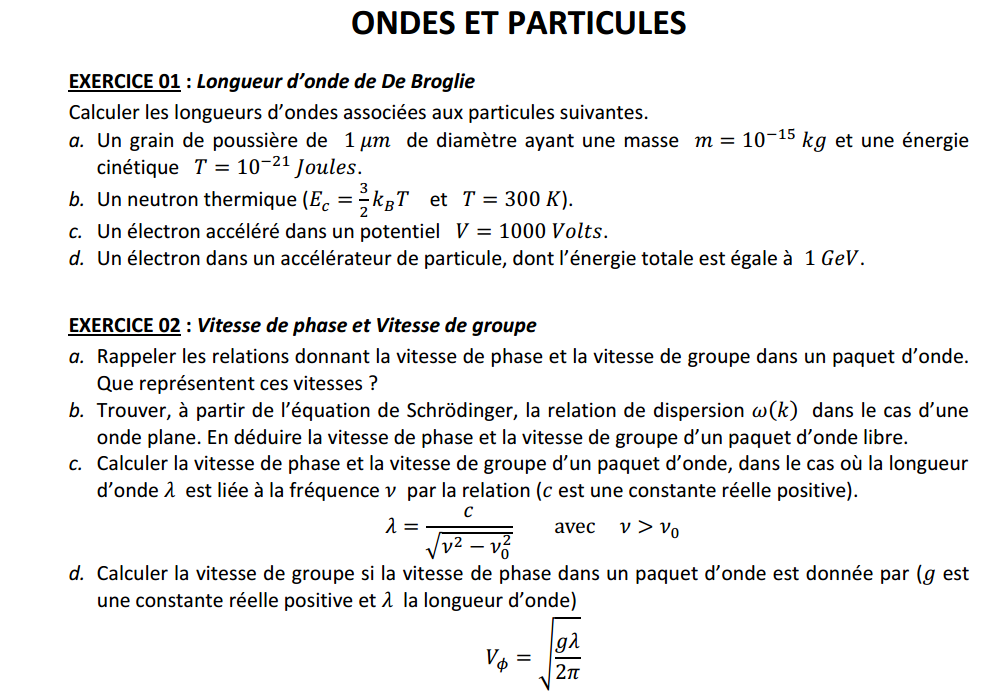
\includegraphics[width=0.9\textwidth]{images/q1.png}
\end{center}
\begin{center}
  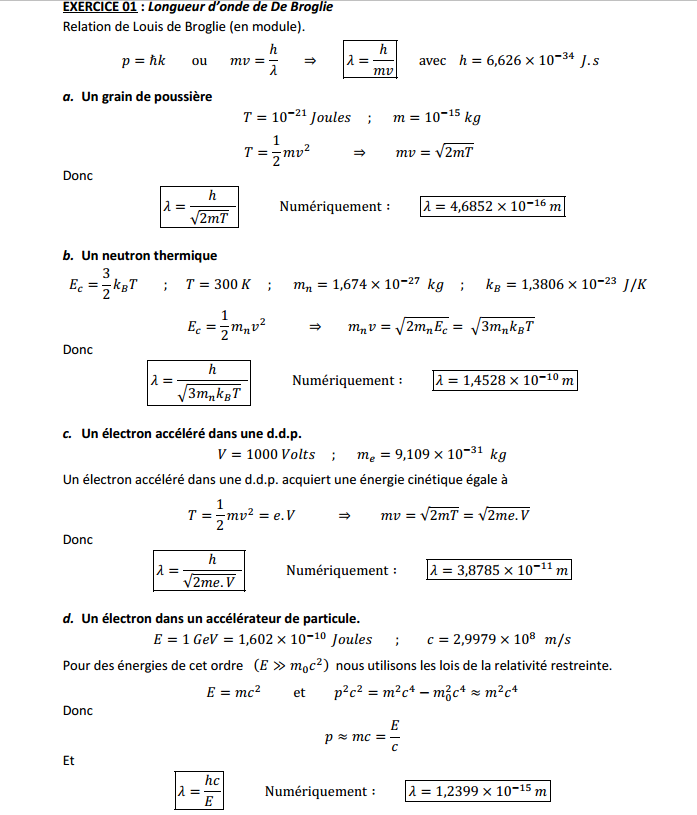
\includegraphics[width=0.9\textwidth]{images/q2.png}
\end{center}
\begin{center}
  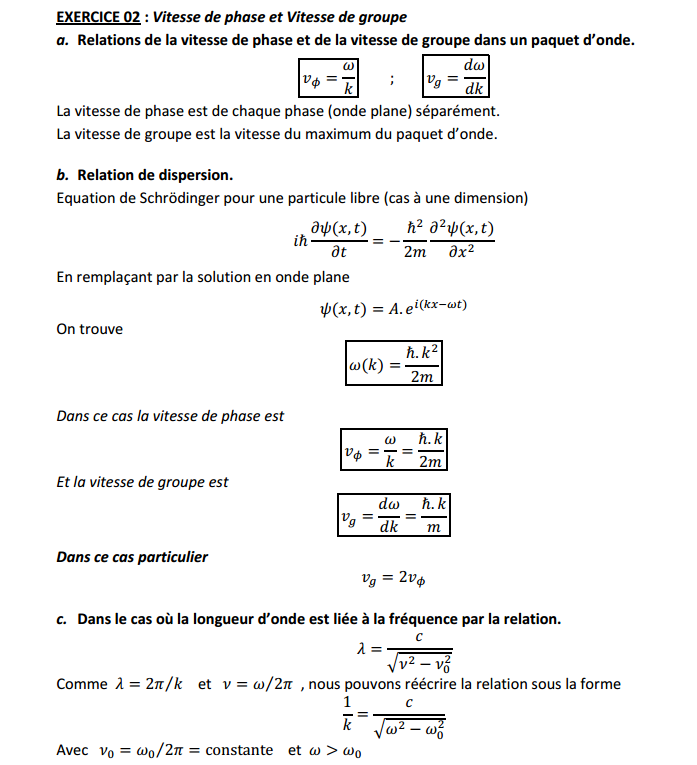
\includegraphics[width=0.9\textwidth]{images/q3.png}
\end{center}
\begin{center}
  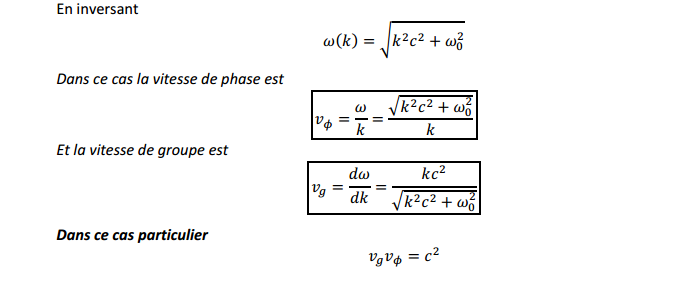
\includegraphics[width=0.9\textwidth]{images/q4.png}
\end{center}
\begin{center}
  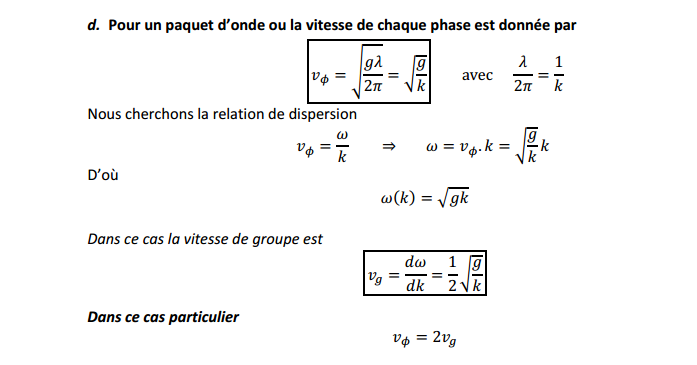
\includegraphics[width=0.9\textwidth]{images/q5.png}
\end{center}
\begin{center}
  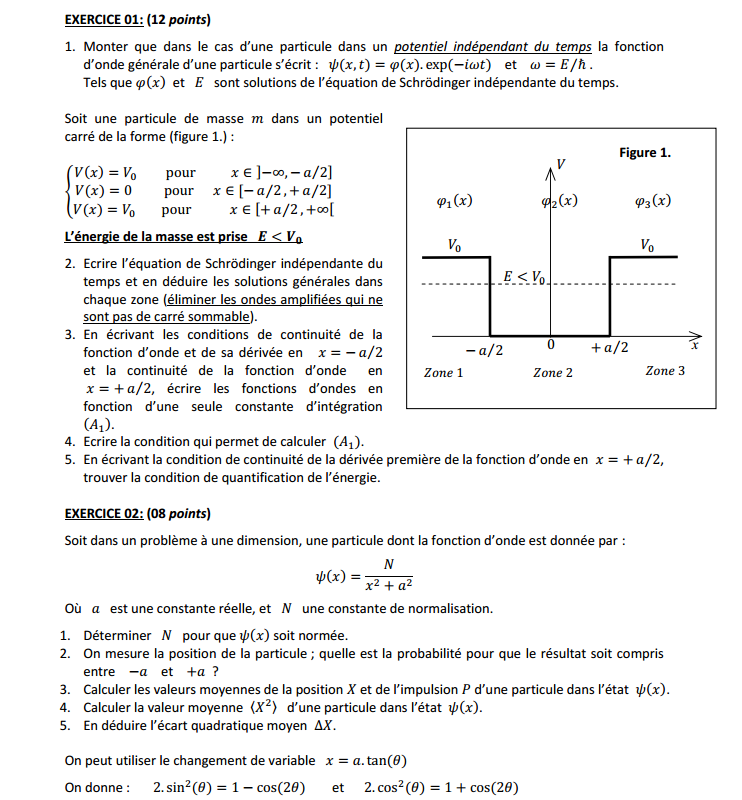
\includegraphics[width=0.9\textwidth]{images/q6.png}
\end{center}
\begin{center}
  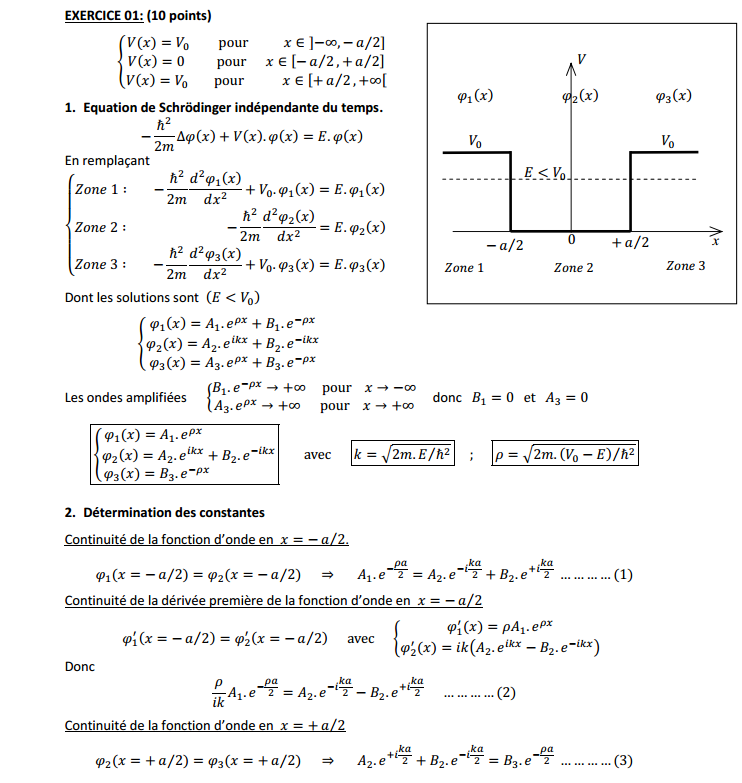
\includegraphics[width=0.9\textwidth]{images/q7.png}
\end{center}
\begin{center}
  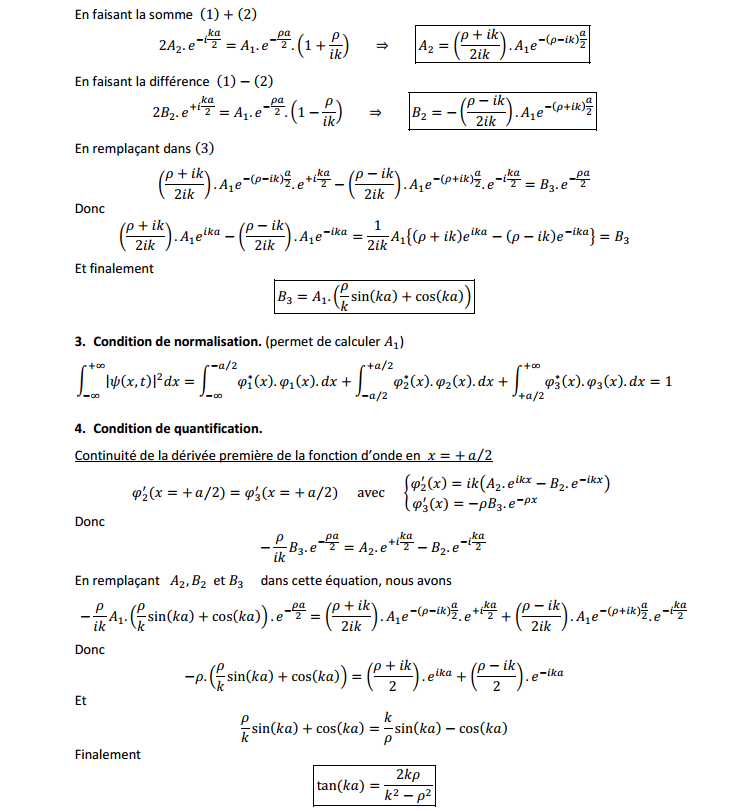
\includegraphics[width=0.9\textwidth]{images/q8.png}
\end{center}

Où $k = \sqrt{2mE/\hbar^2}$ et $\rho = \sqrt{2m(V_0-E)/\hbar^2}$.

\begin{center}
  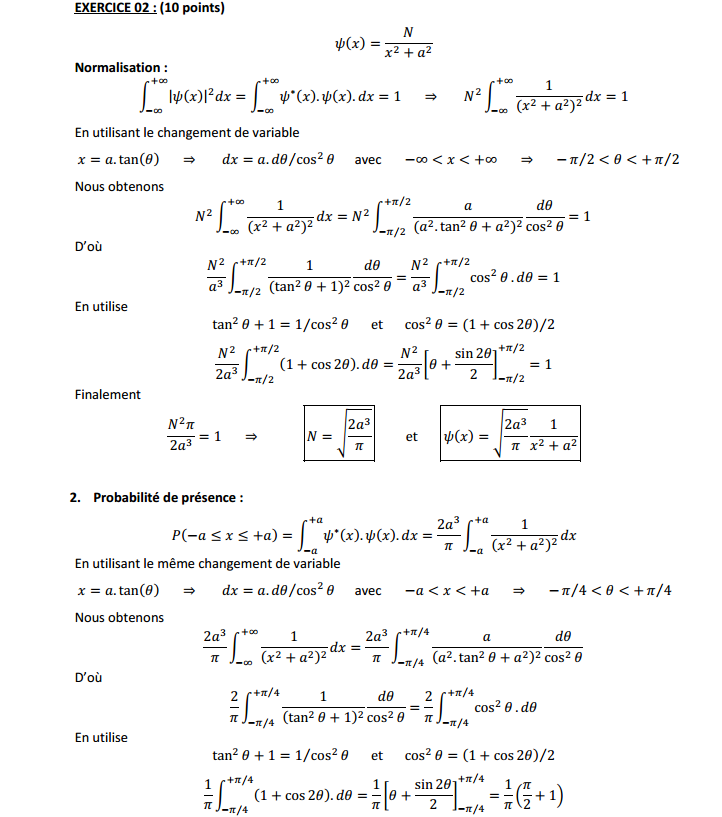
\includegraphics[width=0.9\textwidth]{images/q9.png}
\end{center}
\begin{center}
  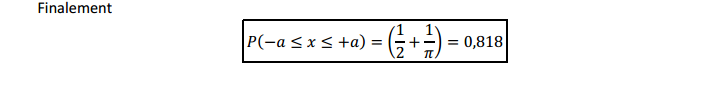
\includegraphics[width=0.9\textwidth]{images/q10.png}
\end{center}
\begin{center}
  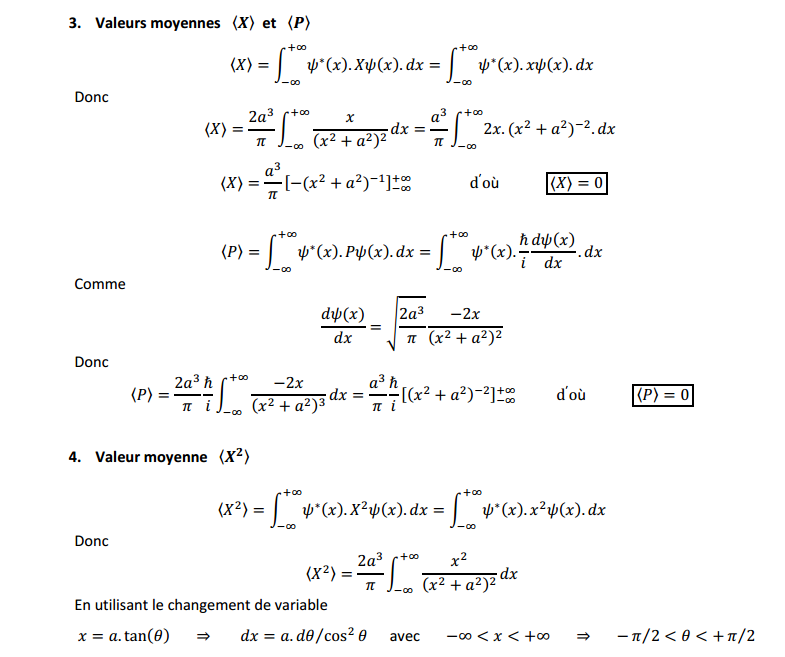
\includegraphics[width=0.9\textwidth]{images/q11.png}
\end{center}
\begin{center}
  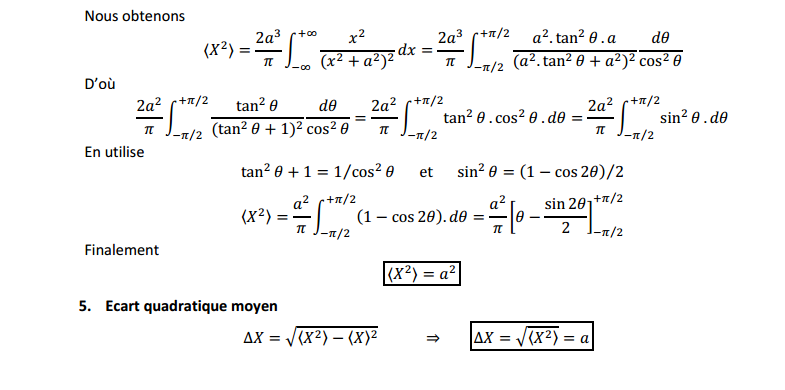
\includegraphics[width=0.9\textwidth]{images/q12.png}
\end{center}
\end{boitecorrige}

\ifdefined\inMainDoc\else\end{document}\fi
